\documentclass[10pt]{beamer}
\usepackage[T1,T2A]{fontenc}
\usepackage[utf8]{inputenc}
\usepackage{hyperref}
\hypersetup{unicode=true}
\usepackage{fontawesome}
\usepackage{graphicx}
\usepackage[english,russian]{babel}
\usepackage{wrapfig}
\usepackage[T1]{fontenc}
\usepackage{fontawesome}
\usepackage{PTSans} 
\mode<presentation>
{
  \usetheme[progressbar=foot,numbering=fraction,background=light]{metropolis} 
  \usecolortheme{default}
  \usefonttheme{default}
  \setbeamertemplate{navigation symbols}{}
  \setbeamertemplate{caption}[numbered]
} 

\let\textttorig\texttt
\renewcommand<>{\texttt}[1]{%
  \only#2{\textttorig{#1}}%
}

\usepackage{minted}

\usepackage{xcolor}
\definecolor{codecolor}{HTML}{FFC300}

\usepackage{tcolorbox}
\tcbuselibrary{most,listingsutf8,minted}

\tcbset{tcbox width=auto,left=1mm,top=1mm,bottom=1mm,
right=1mm,boxsep=1mm,middle=1pt}

\newtcblisting{myr}[1]{colback=codecolor!5,colframe=codecolor!80!black,listing only, 
minted options={numbers=left, style=tcblatex,fontsize=\tiny,breaklines,autogobble,linenos,numbersep=3mm},
left=5mm,enhanced,
title=#1, fonttitle=\bfseries,
listing engine=minted,minted language=r}

\definecolor{mygreen}{HTML}{37980D}
\definecolor{myblue}{HTML}{0D089F}
\definecolor{myred}{HTML}{98290D}

\usepackage{listings}

\lstdefinelanguage{XML}
{
  morestring=[b]",
  morecomment=[s]{<!--}{-->},
  morestring=[s]{>}{<},
  morekeywords={ref,xmlns,version,type,canonicalRef,metr,real,target}
}

\lstdefinestyle{myxml}{
language=XML,
showspaces=false,
showtabs=false,
basicstyle=\ttfamily,
columns=fullflexible,
breaklines=true,
showstringspaces=false,
breakatwhitespace=true,
escapeinside={(*@}{@*)},
basicstyle=\color{mygreen}\ttfamily,
stringstyle=\color{myred},
commentstyle=\color{myblue}\upshape,
keywordstyle=\color{myblue}\bfseries,
}

\title{Приложение <<TODO>>}
\subtitle{Отчет о проектной работе по курсу <<Разработка приложений для мобильных ОС>>}
\author{Д. А. Куусела}
\date{17 января 2022}

\begin{document}

\maketitle

\begin{frame}[fragile]{Цель}
    \begin{block}{Цель работы}

        Разработать мобильное приложение для управления задачами.
    \end{block}
    \begin{block}{Задачи}
        \begin{enumerate}
            \item Организовать хранение данных о задачах
            \item Организовать хранение данных о задачах при выключенном приложении
            \item Разработать интерфейс приложения
            \item Разработать функции для загрузки информации в главный фрагмент
        \end{enumerate}
    \end{block}
\end{frame}

\begin{frame}{Требования к приложению}
    Приложение должно давать пользователю:\\
    \begin{enumerate}
        \item Возможность просматривать текущие задачи
        \item Возможность добавлять новые задачи
        \item Возможность удалять задачи
    \end{enumerate}
\end{frame}

\begin{frame}
    \frametitle{Необходимые классы и функции}
    MainActivity.kt --- главный Kotlin файл, создаёт и запускает Activity.\\
    
    MainFragment.kt --- Kotlin файл, подгружает данные с помощью функции loadTasks, навешивает "прослушку" на кнопку добавления новой задачи. Также в MainFragment есть несколько функций:
    \begin{itemize}
        \item addTask --- преобразование содержимого поля ввода в строку, добавление новой задачи в список, очищение поля ввода;
        \item saveTasks --- сохранение текущих задач в SharedPreferences;
        \item loadTasks --- подгрузка данных из SharedPreferences.  
    \end{itemize}
\end{frame}

\begin{frame}
    CustomAdapter.kt --- Kotlin файл, адаптер между моделью и отображением (view). Функции:
    \begin{itemize}
        \item addTask --- добавление задачи в модель и вызов сохранения данных;
        \item deleteTask --- удаление задачи из модели и вызов сохранения данных;
        \item getTasksList --- возвращает список моделей текущих задач.  
    \end{itemize}
\end{frame}

\begin{frame}[fragile]{Результат}
    \begin{wrapfigure}{l}{0.4\textwidth}
        \vspace{-90pt}
        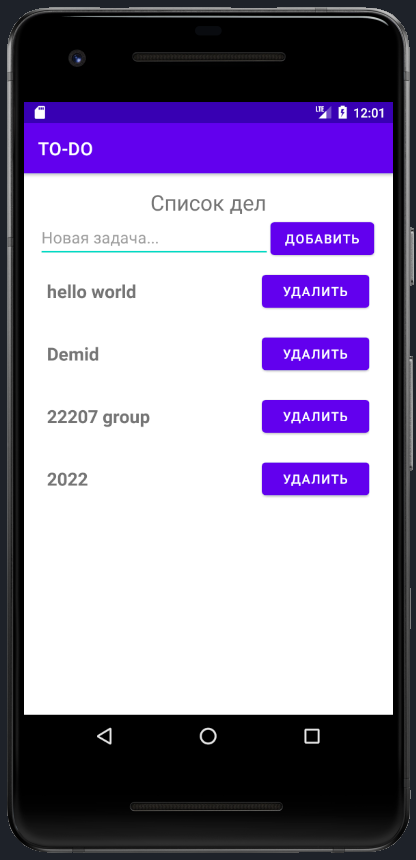
\includegraphics[width = 0.35\textwidth]{images/todoapp.png}
    \end{wrapfigure}
    В результате разработано приложение для просмотра, добавления и удаления текущих задач. Реализованы все запланированные функции. 
        
\end{frame}

\begin{frame}
    \begin{center}
        \Large
        Спасибо за внимание!
    \end{center}
\end{frame}

\end{document}
